
\subsubsection{5.1 RQ1: Structural Break Detection (H-E1)}

PELT detects a single structural break at \textit{paper\_count*} = 39 (breakpoint\_idx = 8, BIC penalty = 4.32).

\textbf{Table 1: H-E1 Primary Results}

\begin{table}[htbp]
\centering
\resizebox{\columnwidth}{!}{%
\begin{tabular}{llll}
\toprule
Metric & Value & Gate Threshold & Status \\
\midrule
Permutation p-value & 0.035 & < 0.05 & PASS \\
paper\_count\* & 39 & $\in$ [10, 120] & PASS \\
Piecewise F-test p-value & 0.0021 & (corroborative) & Strong \\
Bootstrap CI (95\%) & [38, 69.5] & --- & --- \\
n\_bkps detected & 1 & $\geq$ 1 & PASS \\
\bottomrule
\end{tabular}
}
\end{table}

The permutation test asks: if paper\_count labels were randomly shuffled, how often would PELT place a breakpoint at or before index 8? Only 3.5\% of 1000 permutations do so. The piecewise F-test independently confirms: a two-segment model explains data significantly better than a single linear model (F=6.46, p=0.0021). Two fundamentally different tests --- a randomization test on break position and a model comparison --- converge on the same structural break.

\begin{figure}[htbp]
\centering
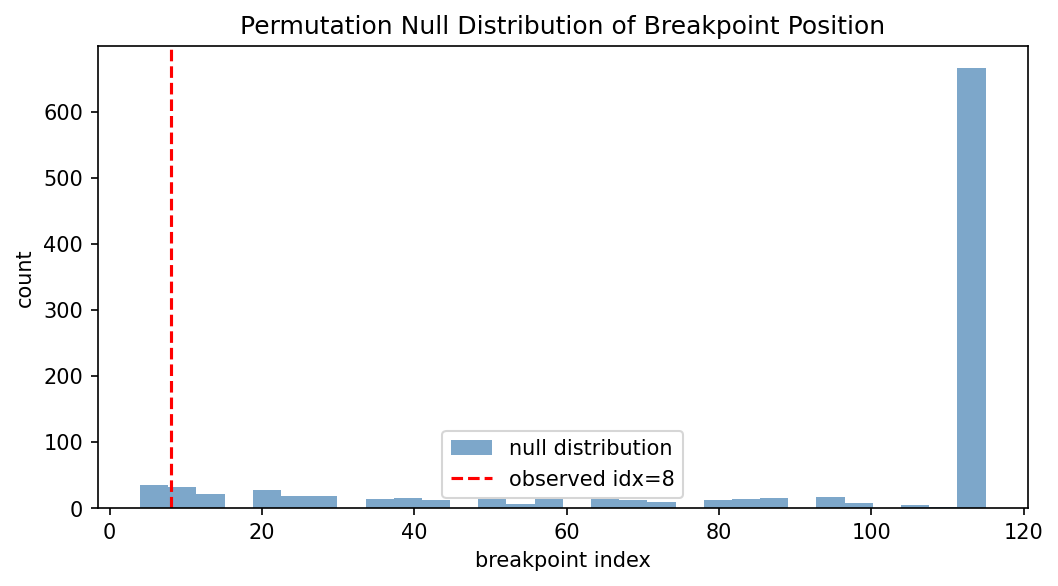
\includegraphics[width=\columnwidth]{figures/fig4_permutation_null.png}
\caption{Permutation null distribution with observed breakpoint at index 8}
\label{fig:fig4_permutation_null}
\end{figure}

\textit{Figure 1. Permutation null distribution of breakpoint positions (1000 shuffles). The observed breakpoint at index 8 (paper\_count=39) falls at the 3.5th percentile of the null distribution.}

\begin{figure}[htbp]
\centering
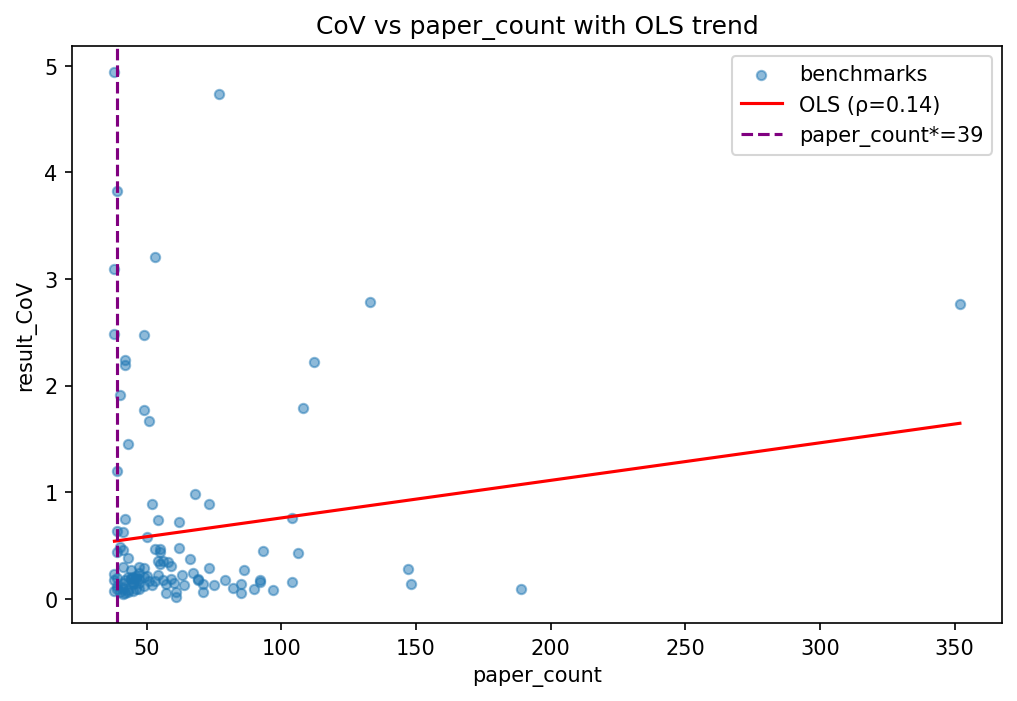
\includegraphics[width=\columnwidth]{figures/fig2_cov_scatter.png}
\caption{CoV vs. paper\_count scatter with breakpoint marker}
\label{fig:fig2_cov_scatter}
\end{figure}

\textit{Figure 2. CoV vs. paper\_count scatter plot with OLS trend line and vertical marker at paper\_count*=39. Benchmarks left of the marker show substantially wider spread than those to the right.}

\begin{figure}[htbp]
\centering
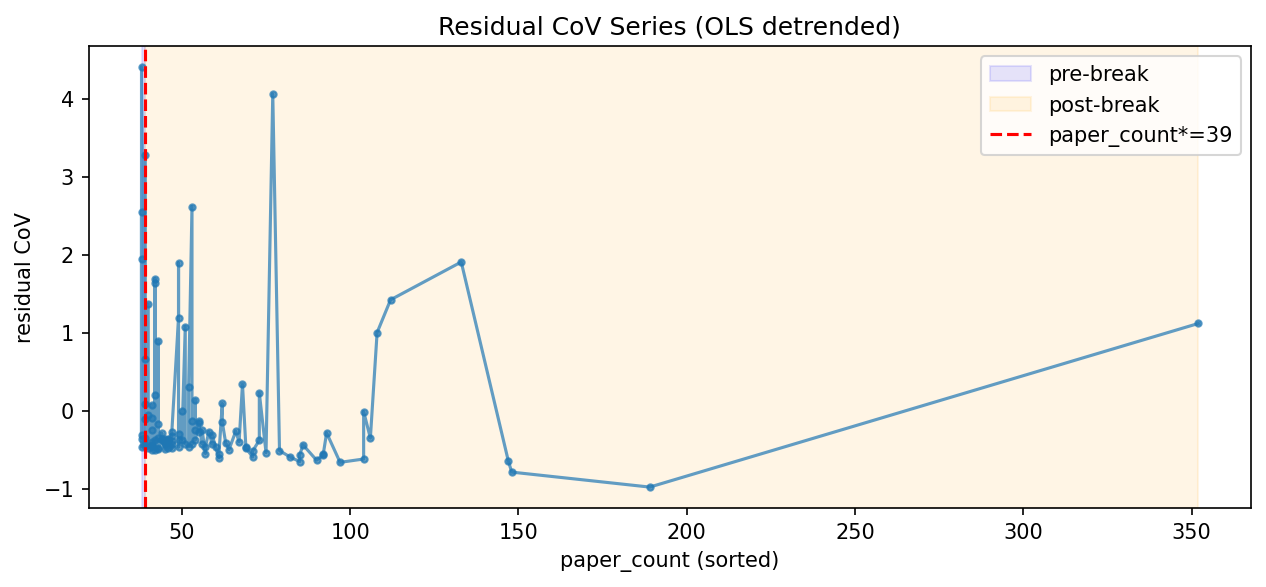
\includegraphics[width=\columnwidth]{figures/fig3_residual_series.png}
\caption{Residual CoV series with pre/post regime shading}
\label{fig:fig3_residual_series}
\end{figure}

\textit{Figure 3. Residual CoV series sorted by paper\_count, with pre-breakpoint (left) and post-breakpoint (right) shading.}

\textbf{OLS trend note:} The global OLS trend is weakly positive (rho = +0.137, $R^{2}=0.019)$. This reverses the rho=$-0.28$ anchor from an earlier snapshot analysis. One plausible explanation is that the dataset composition changed between snapshots (N=111 $\rightarrow$ N=115): newly added benchmarks with high paper\_count and high CoV would locally increase the aggregate trend slope. Per-snapshot benchmark identities are unavailable, so this attribution cannot be confirmed. Importantly, PELT operates on OLS residuals --- after removing whatever linear trend exists --- making the structural break finding robust to trend direction regardless of the reversal's cause.

\begin{figure}[htbp]
\centering
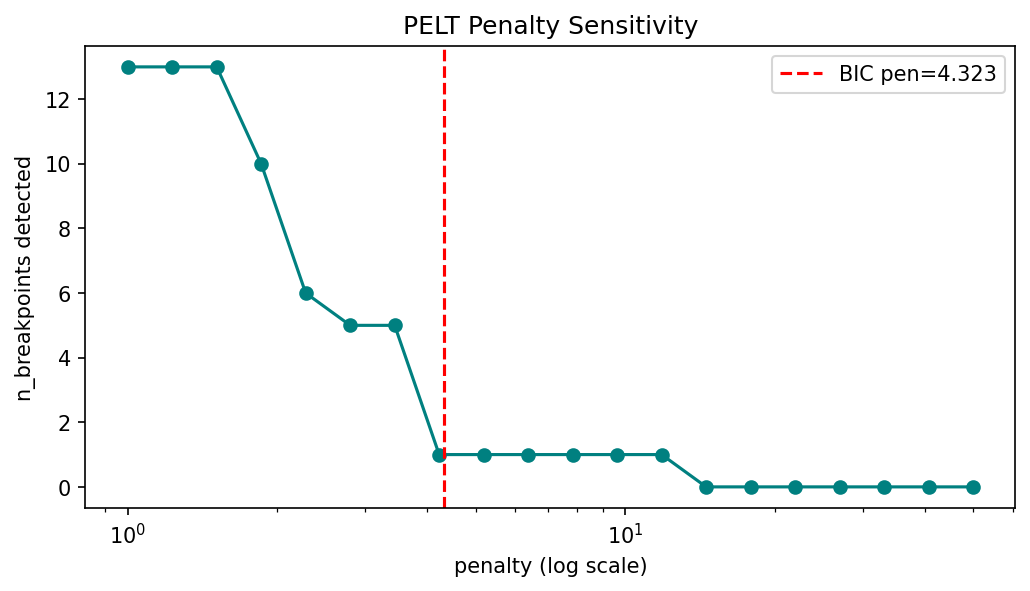
\includegraphics[width=\columnwidth]{figures/fig6_penalty_sensitivity.png}
\caption{PELT penalty sensitivity: breakpoints vs. penalty}
\label{fig:fig6_penalty_sensitivity}
\end{figure}

\textit{Figure 4. PELT breakpoints detected as a function of penalty (log scale). A single breakpoint is confirmed as the stable solution across the relevant penalty range.}

\subsubsection{5.2 RQ2: Exploration Regime Confirmation (H-M1)}

\textbf{Table 2: H-M1 Results --- Exploration Regime}

\begin{table}[htbp]
\centering
\resizebox{\columnwidth}{!}{%
\begin{tabular}{llll}
\toprule
Metric & Value & Gate Threshold & Status \\
\midrule
Global variance & 0.911 & (baseline) & --- \\
Pre-segment variance & 3.475 & > global & PASS \\
Variance ratio (pre/global) & 3.814 & > 1.0 & PASS \\
F-test one-tailed p-value & 0.0009 & < 0.10 & PASS \\
Pre-segment mean residual CoV & +0.873 & > 0 & --- \\
\bottomrule
\end{tabular}
}
\end{table}

The pre-breakpoint segment (n=8) is nearly \textbf{$4\times$ more variable} than the global baseline (F-test p=0.0009). The positive mean residual CoV (+0.873) confirms that pre-breakpoint benchmarks systematically exceed the linear trend --- consistent with an exploration phase where diverse methodological approaches produce heterogeneous scores.

\begin{figure}[htbp]
\centering
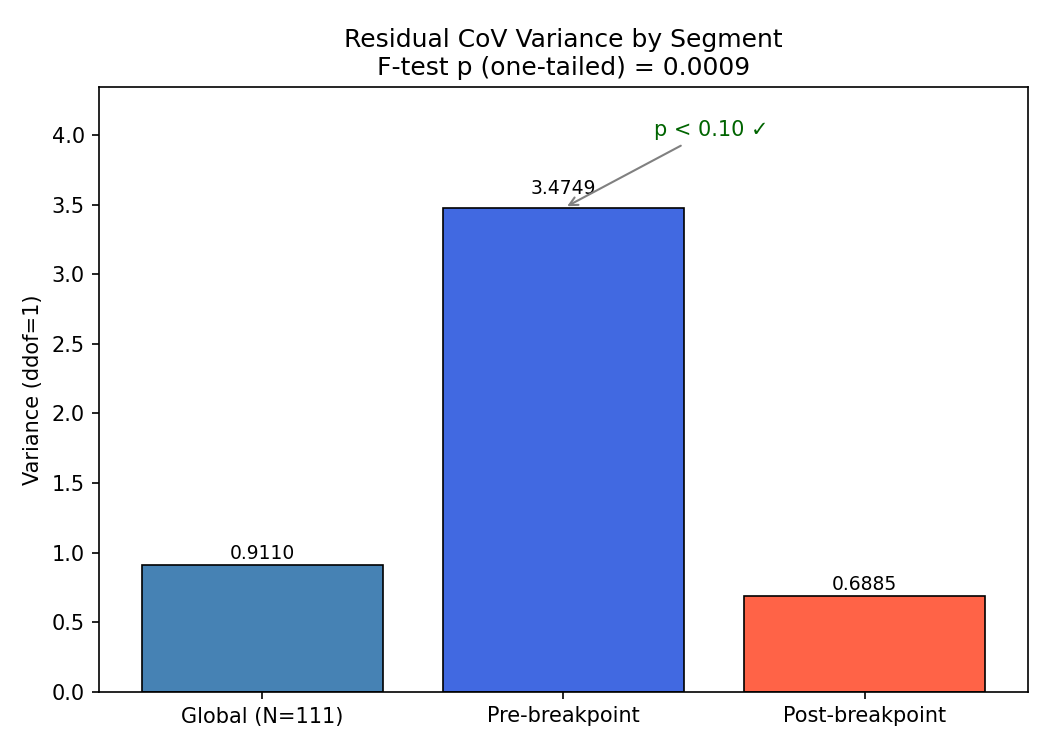
\includegraphics[width=\columnwidth]{figures/fig01_variance_bar.png}
\caption{Pre-segment vs. global baseline variance bar chart}
\label{fig:fig01_variance_bar}
\end{figure}

\textit{Figure 5. Variance bar chart comparing the pre-breakpoint segment (3.475) to the global baseline (0.911). The pre-segment bar is 3.$81\times$ higher.}

\subsubsection{5.3 RQ3: Saturation Compression (H-M2 and H-M3)}

\textbf{Table 3: H-M2 Results --- Saturation Compression}

\begin{table}[htbp]
\centering
\resizebox{\columnwidth}{!}{%
\begin{tabular}{llll}
\toprule
Metric & Value & Gate Threshold & Status \\
\midrule
Pre-segment variance & 3.475 & (reference) & --- \\
Post-segment variance & 0.6885 & < pre & PASS \\
Variance ratio (post/pre) & 0.1981 & < 1.0 & PASS \\
Brown-Forsythe p-value & 0.0099 & < 0.05 & PASS \\
Piecewise F-test p-value & 0.0022 & --- & Significant \\
\bottomrule
\end{tabular}
}
\end{table}

\textit{Note: The piecewise F-test p-value in this table (p=0.0022) differs slightly from the H-E1 value in Table 1 (p=0.0021). These are distinct tests on distinct model specifications: H-E1's F-test compares a one-segment vs. two-segment linear model on the full residual CoV series to confirm break existence; H-M2's F-test compares pre vs. post segment fits within the variance-comparison model. Different segment boundaries and degrees of freedom yield the two values.}

An \textbf{80\% variance reduction} (ratio=0.1981, computed as post-segment relative to pre-segment) after paper\_count\*=39 operationalizes ''saturation'' as a measurable quantity.

\begin{figure}[htbp]
\centering
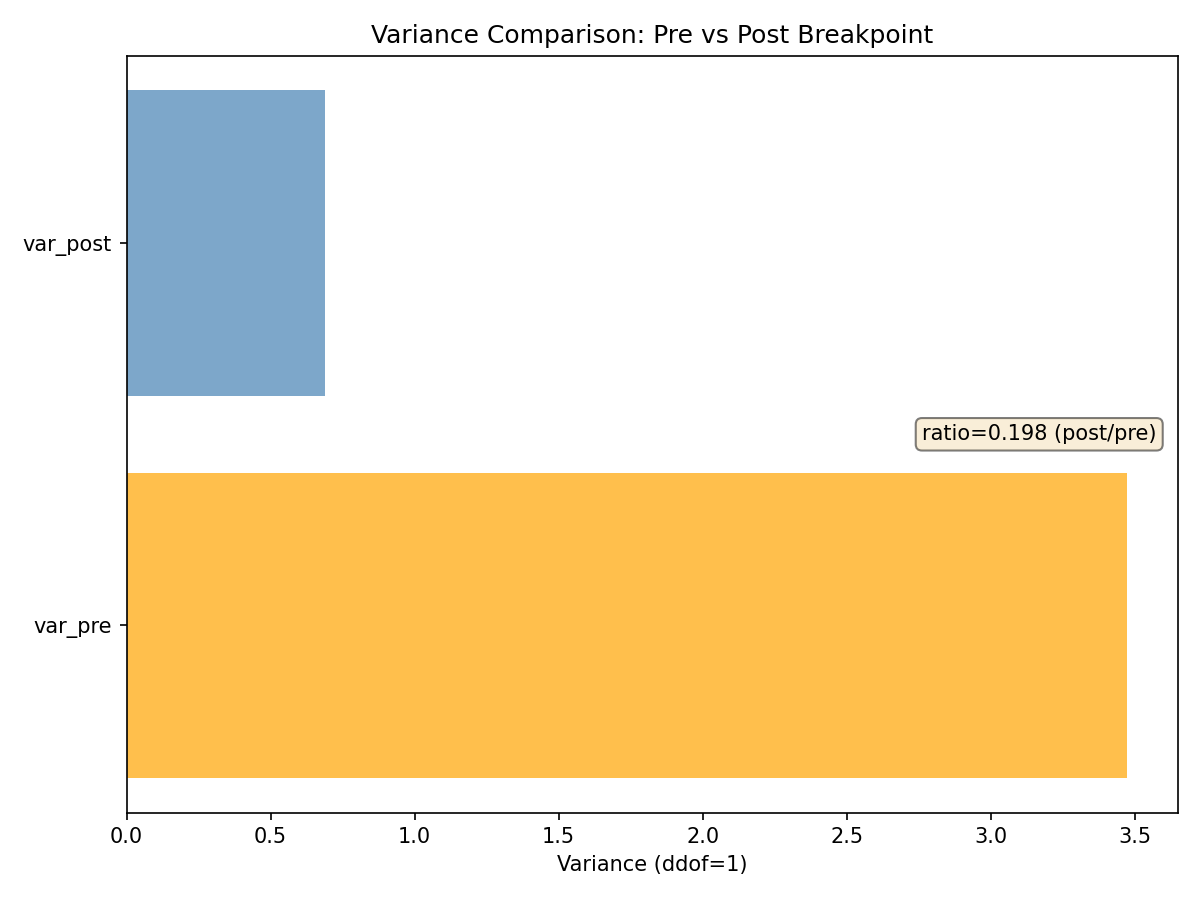
\includegraphics[width=\columnwidth]{figures/variance_bars.png}
\caption{Variance magnitude: pre, post, global}
\label{fig:variance_bars}
\end{figure}

\textit{Figure 6. Variance magnitudes for the pre-breakpoint segment (3.475), post-breakpoint segment (0.6885), and global baseline (0.911).}

\begin{figure}[htbp]
\centering
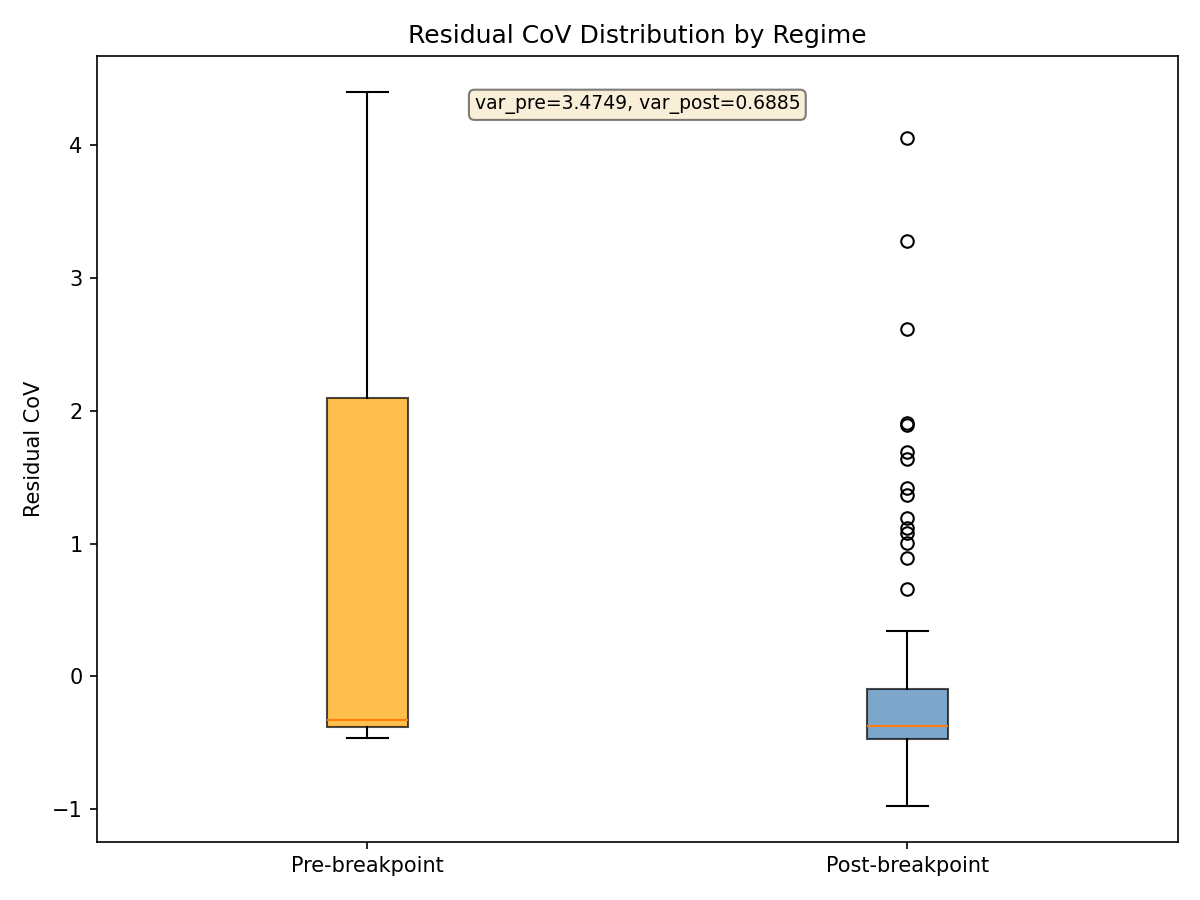
\includegraphics[width=\columnwidth]{figures/boxplots_pre_post.png}
\caption{Pre vs. post residual CoV boxplots}
\label{fig:boxplots_pre_post}
\end{figure}

\textit{Figure 7. Boxplot comparison of residual CoV distributions before and after paper\_count*=39. The post-breakpoint distribution is markedly tighter.}

\textbf{Table 4: H-M3 Directional Metrics}

\begin{table}[htbp]
\centering
\resizebox{\columnwidth}{!}{%
\begin{tabular}{lll}
\toprule
Metric & Result & Status \\
\midrule
M1: Skewness direction (skew\_post < skew\_pre) & skew\_post=2.71 > skew\_pre=1.18 & FAIL \\
M2: Lower-tail (p10\_post < p10\_pre) & p10\_post=$-0.568$ < p10\_pre=$-0.435$ & **PASS** \\
M3: Permutation test on skewness difference & p=0.51 & FAIL \\
M4: Mann-Whitney dominance pre > post & p=0.058 & **PASS** \\
\bottomrule
\end{tabular}
}
\end{table}

M2 and M4 pass the SHOULD\_WORK gate ($\geq 2/4)$. M1 and M3 fail because moment-based estimates on n\_pre=8 have high sampling variance --- a known limitation addressed in §6.2.

\begin{figure}[htbp]
\centering
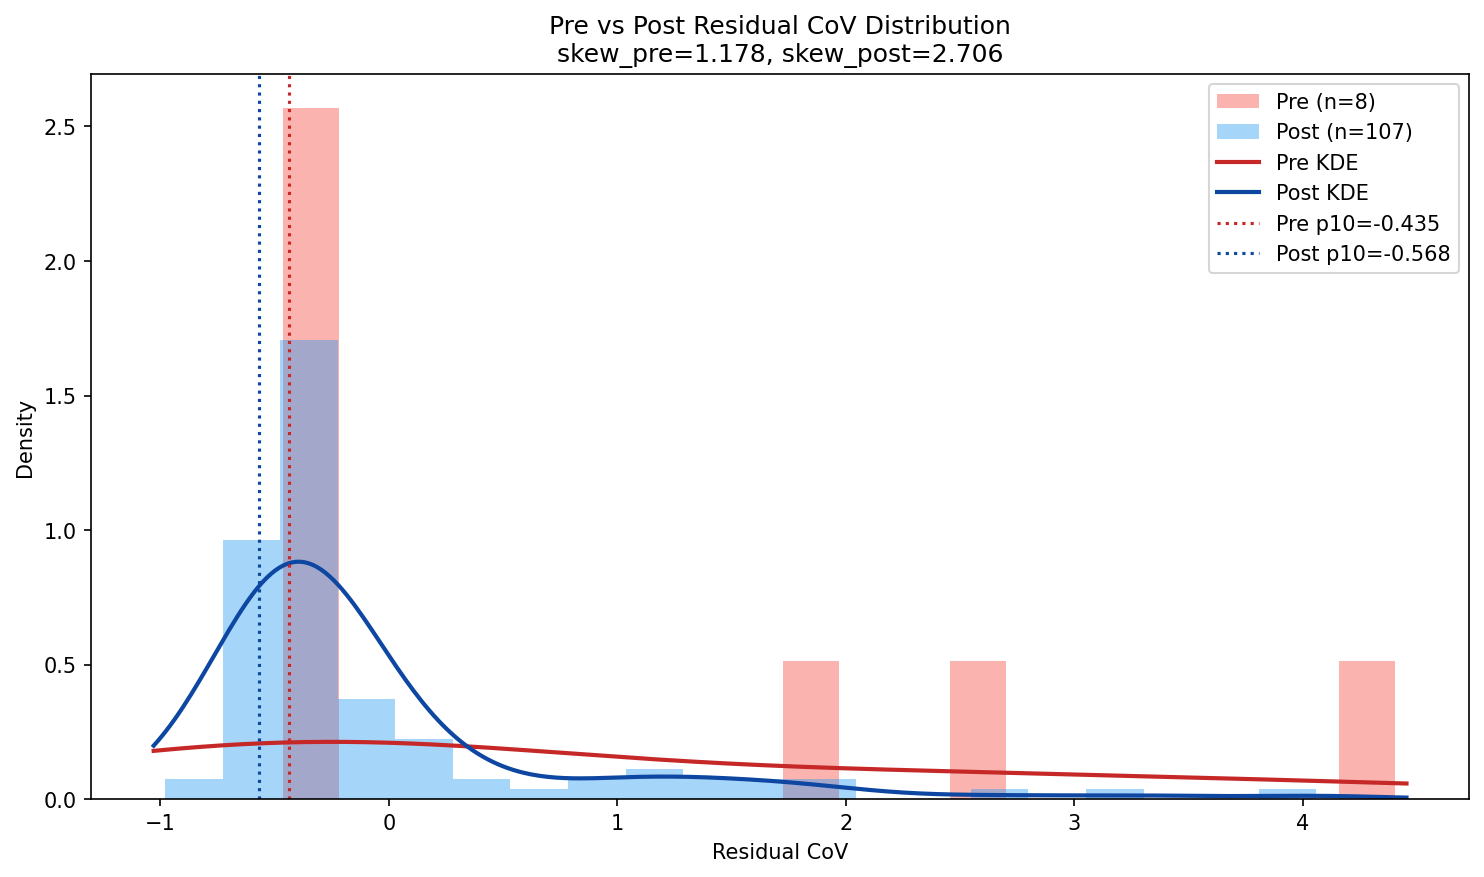
\includegraphics[width=\columnwidth]{figures/histogram_overlay.png}
\caption{Pre/post KDE and histogram with p10 markers}
\label{fig:histogram_overlay}
\end{figure}

\textit{Figure 8. Pre/post residual CoV KDE overlaid on histogram with 10th-percentile markers (p10).}

\subsubsection{5.4 Cross-Experiment Convergence}

\textbf{Table 5: Cross-Experiment Summary}

\begin{table}[htbp]
\centering
\resizebox{\columnwidth}{!}{%
\begin{tabular}{llll}
\toprule
Hypothesis & Gate & Key Evidence & Confidence \\
\midrule
H-E1: Break at paper\_count\*=39 & MUST\_WORK: PASS & Permutation p=0.035, F p=0.0021 & HIGH \\
H-M1: Pre-regime variance 3.$81\times$ global & MUST\_WORK: PASS & F-test p=0.0009 & HIGH \\
H-M2: Post-regime variance $5\times$ lower & MUST\_WORK: PASS & BF p=0.0099, ratio=0.1981 & HIGH \\
H-M3: Post-regime directional concentration & SHOULD\_WORK: PASS (2/4) & 2/4 metrics pass at p<0.10 (M2 + M4); M1 skewness direction and M3 permutation FAIL & MEDIUM \\
\bottomrule
\end{tabular}
}
\end{table}

Three experiments with distinct test designs and null hypotheses converge on the same two-regime narrative. Note that H-E1, H-M1, and H-M2 share the same dataset and the same structural breakpoint (index 8); their convergence reflects consistency of analysis rather than independent replication.

\subsubsection{5.5 Bootstrap Uncertainty}

\begin{figure}[htbp]
\centering
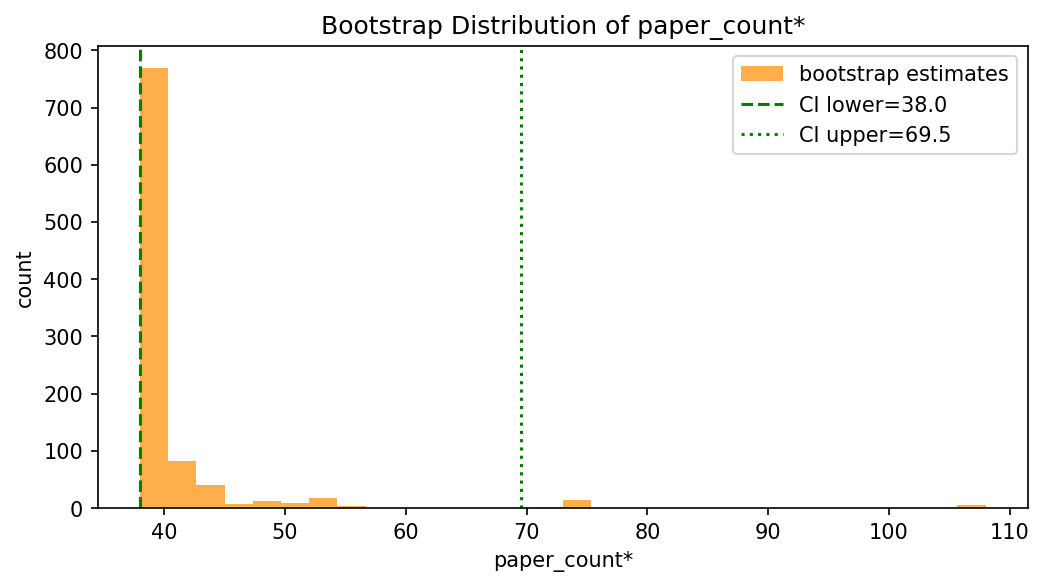
\includegraphics[width=\columnwidth]{figures/fig5_bootstrap_ci.png}
\caption{Bootstrap distribution of paper\_count* with 95\% CI}
\label{fig:fig5_bootstrap_ci}
\end{figure}

\textit{Figure 9. Bootstrap distribution of paper\_count* (1000 resamples). The 95\% CI is [38, 69.5], width=31.5.}

The bootstrap distribution of paper\_count\* (1000 resamples) yields a 95\% CI of [38, 69.5], width=31.5. This width reflects the small pre-segment (n\_pre=8); when 8 observations are resampled with replacement, some bootstrap samples shift the estimate rightward. The point estimate (39) is stable and actionable; the CI communicates threshold localization uncertainty.

\begin{figure}[htbp]
\centering
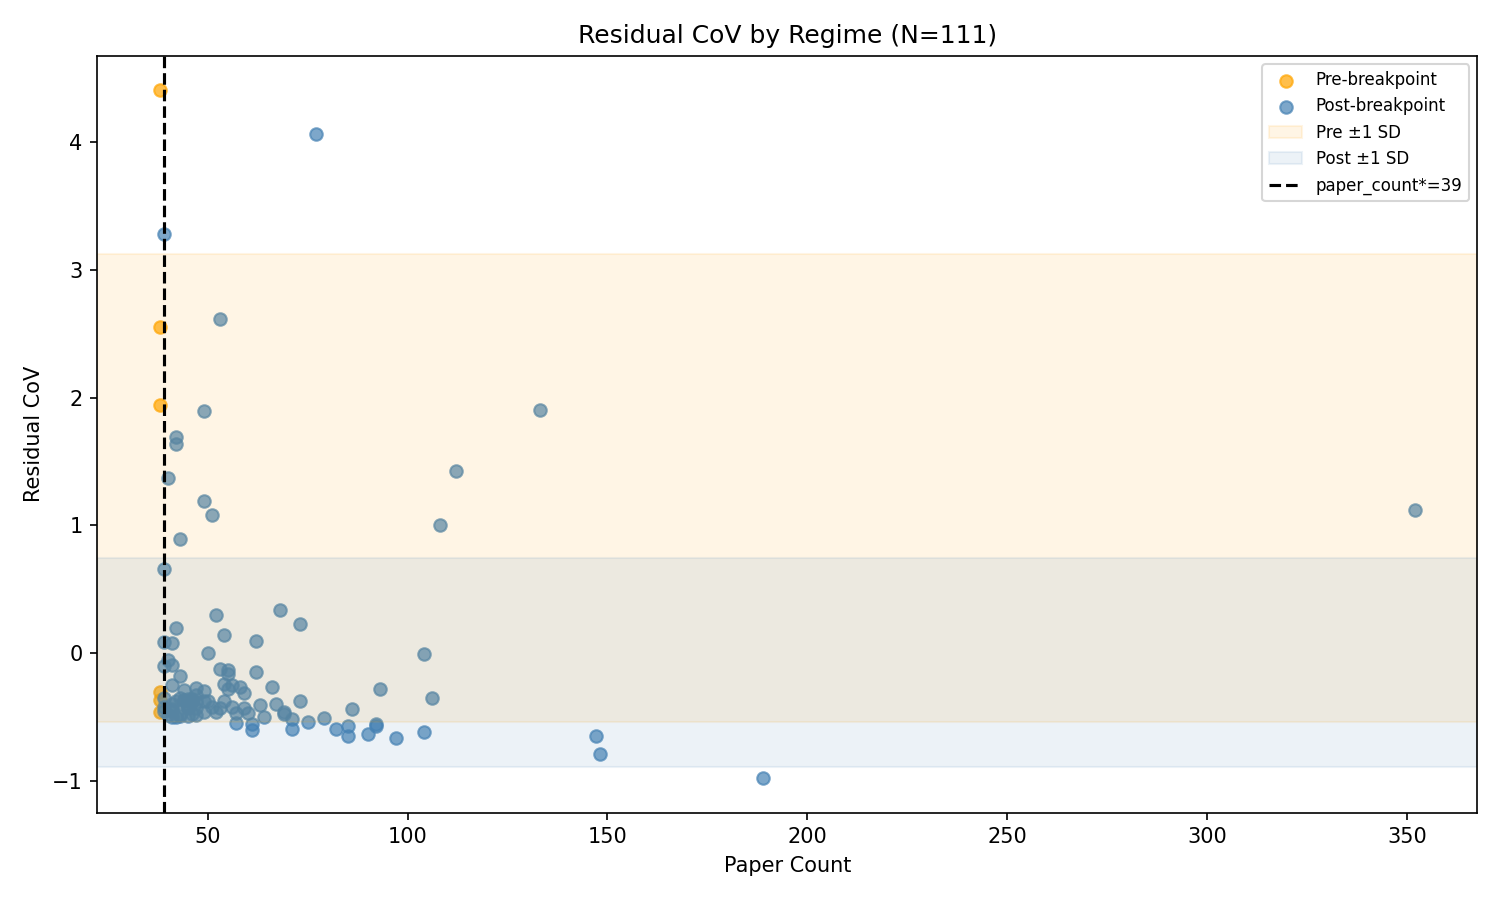
\includegraphics[width=\columnwidth]{figures/scatter_regime.png}
\caption{Residual CoV scatter colored by regime}
\label{fig:scatter_regime}
\end{figure}

\textit{Figure 10. Residual CoV scatter plot with points colored by regime (pre-breakpoint vs. post-breakpoint). The regime separation is visually apparent.}

